Tool and function calling have enabled language models (LMs) to become useful
for tasks beyond just conversation by providing the ability to interact with
external environments and collect further context~\cite{yao2022react, schick2023toolformer, qin2024tool, qu2025tool}. In particular, LM-based
agentic tools and frameworks are often entirely reliant on external tools as
they are designed to interact with the environment to solve some problem or
accomplish a task. Popular agents such as software engineering agents (SWE
agents)~\cite{yang2024swe, liu2024large} need to interact with source code files and the command line to
execute actions. Although access to external tools yields much richer
capabilities and enables LMs to solve long-horizon, real-world tasks, it also
introduces several performance bottlenecks in the traditional inference
pipeline. Instead of a single, contiguous generation, the model alternates
between generation and tool invocation, often across many concurrent sessions,
resulting in gaps due to waiting on tool completion.

\begin{figure}[h]
    \centering
    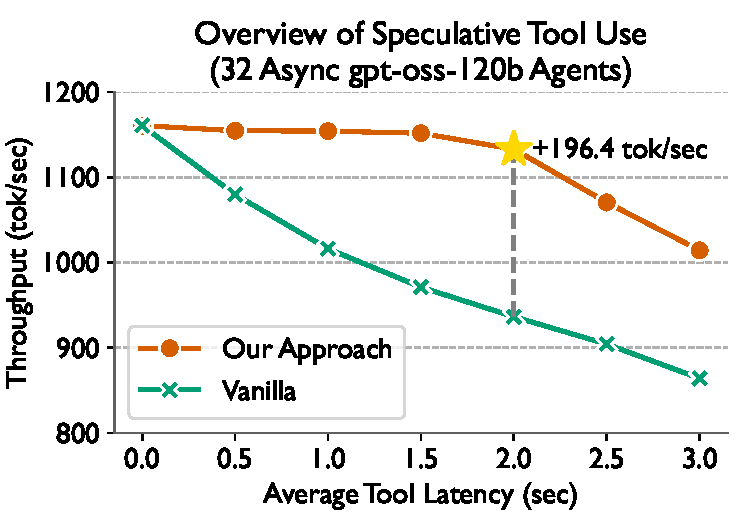
\includegraphics[width=0.95\linewidth]{figs/results-overview}
    \caption{Our approach leads to up to 196 tokens/second improvement in the vLLM server when there are 32 gpt-oss-120b agents using it for inference. \label{fig:results-intro}}
\end{figure}

As tool-centric agents become more prevalent in code co-pilots, personal
assistants, and autonomous workflows, the overhead of using these agents is
increasingly dominated by the time spent waiting on tools.  Each tool call forces generation to stop and return to the user, who handles running the tool and sending back its output. This interrupt-driven process introduces a strict sequential dependency, where the latencies of individual tool calls accumulate and can significantly increase total generation time. Additionally, the evicted sequences and tool output must be rescheduled back into the inference engine, causing further overhead. Even with optimizations such as prefix-caching~\cite{kwon2023efficient, vllm_apc, zheng2024sglang, gao2024cost}, there are still significant overheads to removing the sequences, processing the tool output, and rescheduling them for generation. These overheads are further exacerbated in multi-tenant settings where scheduling and prefix-caching optimizations become more challenging with many agents contending for resources, and many concurrent prompts evicting existing entries in the KV-cache. Removing the sequential dependence and reducing these overheads in tool-heavy workloads is critical as agentic LMs become more widespread and need to be more economically viable and efficient.


Breaking the strict sequential dependency introduced by tool calls and reducing eviction overheads is non-trivial from a systems perspective.
Tool latencies can span orders of magnitude and depend
on external services, filesystem I/O, or user-defined code, making them
difficult to predict or bound.  
Long-running tools inevitably dominate end-to-end latency, whereas for short tools, the overheads of eviction and re-entry into the engine can outweigh any potential latency hiding strategies.
Furthermore, decoupling tool execution from model progression introduces correctness challenges, and naively running tools early or out of order can lead to wasted computation with unused results or outputs that are inconsistent with the model’s eventual decisions.
Finally, existing inference optimizations such as speculative decoding~\cite{leviathan_fast_2023, chen2023accelerating} and optimized KV-cache management~\cite{kwon2023efficient}
are implemented entirely within the inference engine and treat tools as opaque
interruptions, making it difficult for client-side innovations to impact
engine performance.


We address these challenges in agent tool calling by introducing \emph{speculative tool execution}, realized through two variants. First, we present a client-side strategy that breaks the sequential nature of tool execution without requiring any modifications to the inference engine, making it immediately compatible with existing inference services. Second, we introduce an engine-level mechanism that enables the inference system to ingest tool outputs directly and eliminate eviction-related overheads. These strategies allow us to mask portions of tool execution with generation for stateless and cheap-to-execute tools.
Furthermore, we provide an analytical performance model for both approaches and discuss the impact of tool durations, prediction accuracies,
and decode latencies on the performance improvements. The proposed
approaches are evaluated across a range of workloads, demonstrating up to
several hundred tokens per second throughput improvements.
\Cref{fig:results-intro} highlights the savings of our approach over standard inference with tool calling agents.

In this work, we make the following important contributions:
\begin{itemize}
    \item Two novel methods for speculating tool calls to optimize inference for agents by speculating work and keeping prompts resident in the engine.
    \item A theoretical analysis on the limitations of our methods, and which configurations will yield highest performing results.
    \item A detailed study of our two methods on agent workflows with tool calling.
\end{itemize}
